% ----------------------------------------------------------------- %
% TEMPLATE AUTHOR .... Steven E. Thornton                           %
% MC AUTHOR .... Kamil S. Jaron                                     %
% CONTACT ... kamiljaron@gmailcom                                   %
% TEMPLATE ARTICLE ... steventhornton.ca/markov-chains-in-latex/    %
% ----------------------------------------------------------------- %
\documentclass{standalone}

\usepackage{tikz}
\usetikzlibrary{automata, positioning}

\begin{document}
    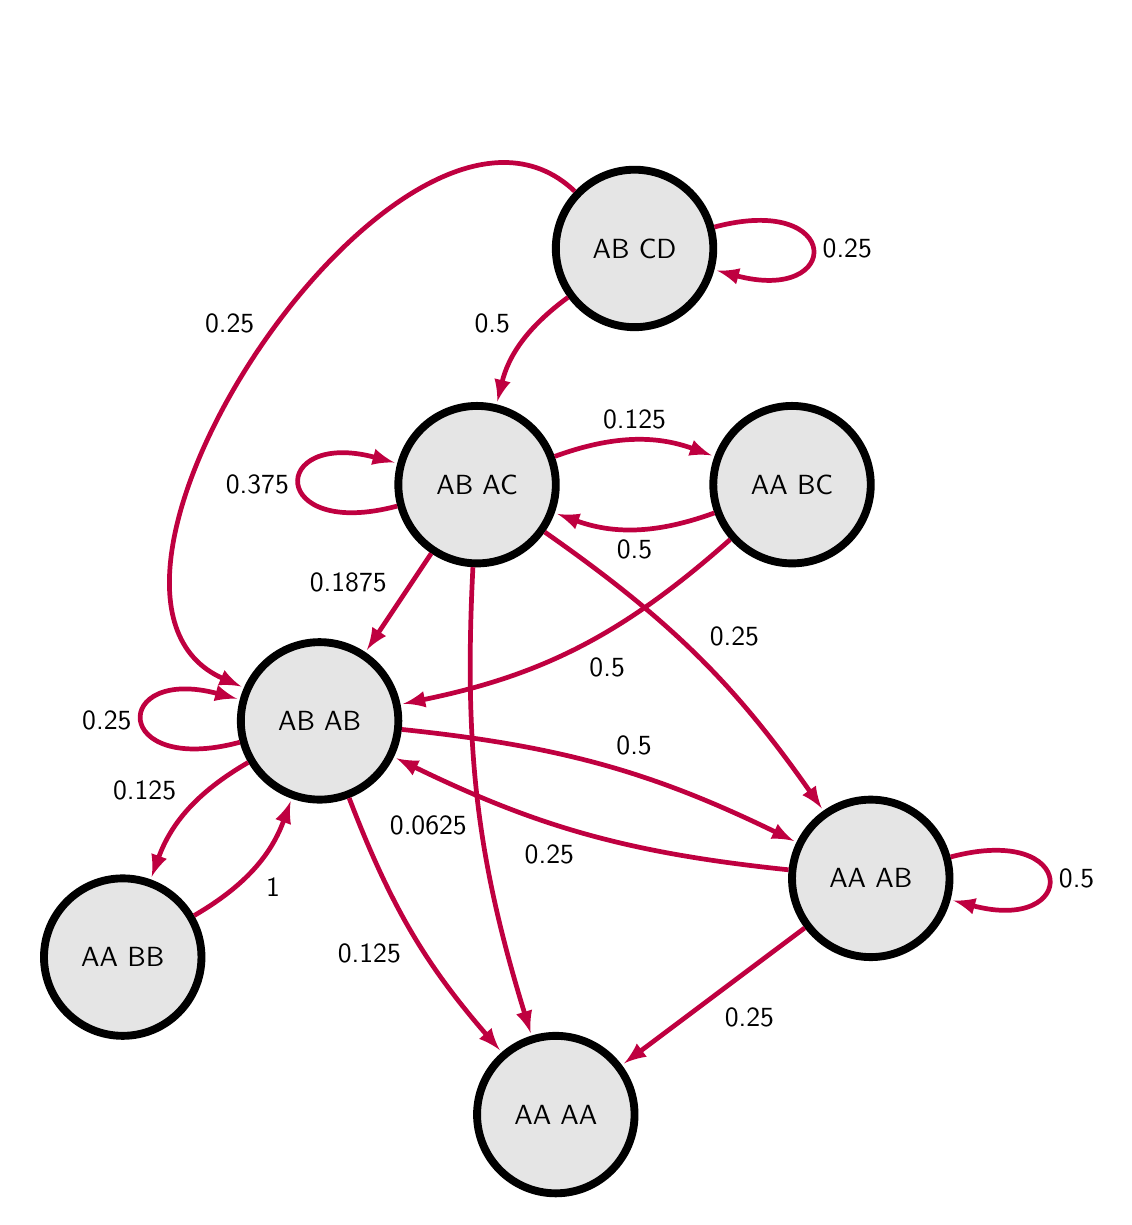
\begin{tikzpicture}[font=\sffamily]

        % Setup the style for the states
        \tikzset{node style/.style={state,
                                    minimum width=2cm,
                                    line width=1mm,
                                    fill=gray!20!white}}

        % Draw the states
        % c('AB  CD', 'AB  AC', 'AA  BC', 'AB  AB', 'AA  AB', 'AA  BB'),
        \node[node style] at (0, 10)      (abcd)     {AB CD};

        \node[node style] at (-2, 7)      (abac)     {AB AC};
        \node[node style] at (2, 7)       (aabc)     {AA BC};

        \node[node style] at (-4, 4)      (abab)     {AB AB};
        \node[node style] at ( 3, 2)       (aaab)     {AA AB};
        \node[node style] at (-6.5, 1)       (aabb)     {AA BB};

        \node[node style] at (-1, -1)       (aaaa)     {AA AA};

        % Connect the states with arrows
        \draw[every loop,
              auto=right,
              line width=0.6mm,
              >=latex,
              draw=purple,
              fill=purple]
            (abcd)     edge[loop right]             node {0.25} (abcd)
            (abcd)     edge[bend right=20]          node {0.5} (abac)
            (abcd)     edge[bend right=100]         node {0.25} (abab)
            % AB AC
            (abac)     edge[loop left]                node {0.375} (abac)
            (abac)     edge[bend left=20, auto=left]  node {0.125}  (aabc)
            (abac)     edge[bend right=0]             node {0.1875} (abab)
            (abac)     edge[bend left=10, auto=left]  node {0.25} (aaab)
            (abac)     edge[bend right=10]            node {0.0625} (aaaa)
            % AA BC
            (aabc)     edge[bend left=15, auto=left]         node {0.5} (abab)
            (aabc)     edge[bend left=20, auto=left]         node {0.5}  (abac)
            % AB AB
            (abab)     edge[loop left, auto=left]    node {0.25} (abab)
            (abab)     edge[bend left=10, auto=left]  node {0.5} (aaab)
            (abab)     edge[bend right=20]            node {0.125} (aabb)
            (abab)     edge[bend right=10]            node {0.125} (aaaa)
             % AA AB
            (aaab)     edge[bend left=10, auto=left]       node {0.25} (abab)
            (aaab)     edge[loop right]                    node {0.5} (aaab)
            (aaab)     edge[bend right=0, auto=left]       node {0.25} (aaaa)
             % AA BB
            (aabb)     edge[bend right=20, auto=right]            node {1} (abab);
             % AA AA
            (aaaa)     edge[loop right, auto=left]            node {1} (aaaa);


%  abac	aabc	abab	2aaab	2aabb	1aaaa

    \end{tikzpicture}
\end{document}